% Figure 4.4. 2D Bearing device design domain and boundary conditions.
% Build in WSL: pdflatex for PDF, pdftocairo -png -r 300 for PNG.
\documentclass[tikz,border=3pt]{standalone}
\usepackage{amsmath}
\usepackage{tikz}
\usetikzlibrary{arrows.meta}

\begin{document}
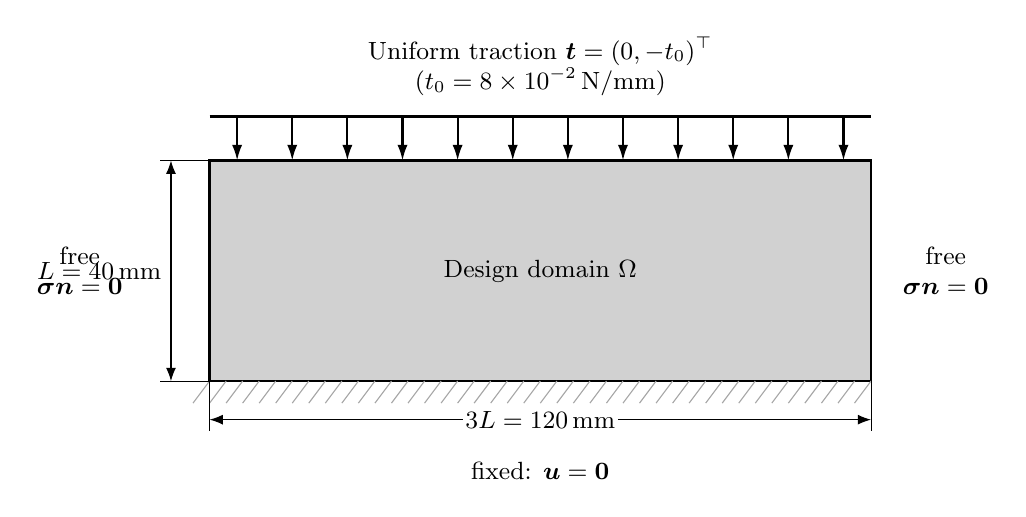
\begin{tikzpicture}[x=0.07cm,y=0.07cm,>=Latex]
  \def\L{120}
  \def\H{40}

  % ================= 设计域矩形 =================
  \draw[thick,fill=black!18] (0,0) rectangle (\L,\H);

  % ================= 底部固支边界与阴影线 =================
  \draw[thick] (0,0) -- (\L,0);
  \foreach \x in {0,3,...,120} {
    \draw[gray!70] (\x,0) -- (\x-3,-4);
  }
  \node[font=\small,align=center,anchor=north] at (0.5*\L,-13)
    {fixed: $\boldsymbol{u}=\boldsymbol{0}$};

  % ================= 顶部均布压力载荷 =================
  \draw[thick] (0,\H+8) -- (\L,\H+8);
  \foreach \x in {5,15,...,115} {
    \draw[thick,-{Latex[length=2.0mm,width=1.3mm]}] (\x,\H+8) -- (\x,\H);
  }
  \node[font=\small,align=center,anchor=south] at (0.5*\L,\H+10)
    {Uniform traction $\boldsymbol{t}=(0,-t_0)^\top$\\($t_0 = 8\times 10^{-2}\,\mathrm{N/mm}$)};

  % ================= 尺寸标注 =================
  % 宽度标注 (放在底部阴影线与文字之间)
  \draw[thin] (0,0) -- (0,-9);
  \draw[thin] (\L,0) -- (\L,-9);
  \draw[<->,thin] (0,-7) -- (\L,-7)
    node[midway,fill=white,inner sep=1pt,font=\small] {$3L=120\,\mathrm{mm}$};

  % 高度标注 (放在左侧)
  \draw[thin] (0,0) -- (-9,0);
  \draw[thin] (0,\H) -- (-9,\H);
  \draw[<->,thin] (-7,0) -- (-7,\H)
    node[midway,left,font=\small] {$L=40\,\mathrm{mm}$};

  % ================= 自由边界与域标注 =================
  \node[font=\small,align=center,anchor=east] at (-14,0.5*\H)
    {free\\$\boldsymbol{\sigma}\boldsymbol{n}=\boldsymbol{0}$};

  \node[font=\small,align=center,anchor=west] at (\L+4,0.5*\H)
    {free\\$\boldsymbol{\sigma}\boldsymbol{n}=\boldsymbol{0}$};

  \node[font=\small,align=center] at (0.5*\L,0.5*\H)
    {Design domain $\Omega$};

\end{tikzpicture}
\end{document}
